% CS615 Aspects of System Administration
% Author: Jan Schaumann <jschauma@netmeister.org>
% $Id: slides.tex,v 1.6 2006/03/07 13:55:55 jschauma Exp $

\documentclass[xga]{xdvislides}
\usepackage[landscape]{geometry}
\usepackage{graphics}
\usepackage{graphicx}
\usepackage{colordvi}

\begin{document}
\setfontphv

%%% Headers and footers
\lhead{\slidetitle}                               % default:\lhead{\slidetitle}
\chead{CS615 - Aspects of System Administration}% default:\chead{\relax}
\rhead{Slide \thepage}                       % default:\rhead{\sectiontitle}
\lfoot{\Gray{Performance Tuning Basics; SMTP}}% default:\lfoot{\slideauthor}
\cfoot{\relax}                               % default:\cfoot{\relax}
\rfoot{\Gray{\today}}

\vspace*{\fill}
\begin{center}
	\Hugesize
		CS615 - Aspects of System Administration\\ [1em]
		Performance Tuning Basics; SMTP \\ [1em]
	\hspace*{5mm}\blueline\\ [1em]
	\Normalsize
		Department of Computer Science\\
		Stevens Institute of Technology\\
		Jan Schaumann\\
		\verb+jschauma@stevens-tech.edu+
		\verb+http://www.cs.stevens-tech.edu/~jschauma/615/+
\end{center}
\vspace*{\fill}

\subsection{Symptoms}
\vspace{.5in}
\begin{center}
	\Huge
	``The system feels slow.''
\end{center}
\Normalsize

\subsection{Symptoms}
\vspace{.5in}
\begin{center}
	\Huge
	``How much time does it take to run my job?''
\end{center}
\Normalsize

\subsection{Symptoms}
\begin{center}
	
\includegraphics[scale=0.7]{pics/wall-clock.eps}
\end{center}

\subsection{Diagnosis}
\vspace{.5in}
\begin{center}
	\Huge
	Know your applications. \\
\end{center}
\Normalsize

\subsection{Diagnosis}
\vspace{.5in}
\begin{center}
	\Huge
	Know your applications. \\
	\vspace{.4in}
	Know your users. \\
\end{center}
\Normalsize

\subsection{Diagnosis}
\vspace{.5in}
\begin{center}
	\Huge
	Know your applications. \\
	\vspace{.4in}
	Know your users. \\
	\vspace{.4in}
	Know your traffic patterns. \\
\end{center}
\Normalsize

\subsection{Diagnosis}
\vspace{.5in}
\begin{center}
	\Huge
	Know your applications. \\
	\vspace{.4in}
	Know your users. \\
	\vspace{.4in}
	Know your traffic patterns. \\
	\vspace{.4in}
	{\em Know your systems.}
\end{center}
\Normalsize

\subsection{Diagnosis}
\begin{center}
	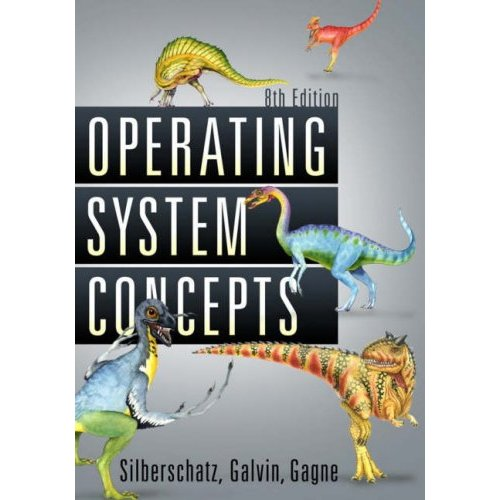
\includegraphics[scale=0.7]{pics/silberschatz.eps}
\end{center}

\subsection{Monitoring System Activity}
\vspace{.5in}
\begin{center}
	\Huge
	``How much time does it take to run my job?'' \\
	\vspace{.5in}
	\verb+/usr/bin/time <application>+ \\
\end{center}
\Normalsize

%\subsection{Diagnosis}
%\begin{center}
%	\includegraphics[scale=1.0]{pics/time-is-relative.eps}
%\end{center}
%
%
%\subsection{Diagnosis}
%\begin{center}
%	\includegraphics[scale=1.0]{pics/DaliProfileOfTime.eps} \\
%	``Profile of Time''
%\end{center}
%
%\subsection{Diagnosis}
%\begin{center}
%	\includegraphics[scale=0.7]{pics/persistence_of_time.eps} \\
%	``Persistence of Memory''
%\end{center}
%
%\subsection{Diagnosis}
%\begin{center}
%	\includegraphics[scale=0.7]{pics/persistence_of_time2.eps}
%\end{center}

\subsection{Diagnosis}
\begin{verbatim}
$ time dd if=/dev/urandom of=a bs=1MB count=25 2>/dev/null

real	0m3.12s
user	0m0.00s
sys	0m3.07s
$
\end{verbatim}

\subsection{Diagnosis}
\begin{verbatim}
$ time dd if=/dev/urandom of=a bs=1MB count=25 2>/dev/null

real	0m3.12s
user	0m0.00s
sys	0m3.07s
$ time dd if=/dev/urandom bs=1MB count=25 2>/dev/null | wc >/dev/null

real	0m4.17s
user	0m1.08s
sys	0m3.05s
$
\end{verbatim}

\subsection{Diagnosis}
\begin{verbatim}
$ time dd if=/dev/urandom of=a bs=1MB count=25 2>/dev/null

real	0m3.12s
user	0m0.00s
sys	0m3.07s
$ time dd if=/dev/urandom bs=1MB count=25 2>/dev/null | wc >/dev/null

real	0m4.17s
user	0m1.08s
sys	0m3.05s
$ time dd if=/dev/zero of=b bs=1MB count=25 2>/dev/null

real	0m0.06s
user	0m0.00s
sys	0m0.05s
$
\end{verbatim}


\subsection{Diagnosis}
\begin{verbatim}
$ dd if=/dev/zero of=a bs=1MB count=500 >/dev/null 2>&1
$ time cp a b

real	0m1.25s
user	0m0.02s
sys	0m1.03s
$ time mv b c

real	0m0.01s
user	0m0.01s
sys	0m0.00s
$ time rm [ac]

real	0m0.16s
user	0m0.00s
sys	0m0.16s
$
\end{verbatim}

\subsection{Know your systems.}
Useful tools:
\begin{itemize}
	\item simple:
		\begin{itemize}
			\item cron(8)
			\item ps(1) / top(1)
			\item time(1)
			\item uptime(1) / w(1)
		\end{itemize}
	\item more advanced:
		\begin{itemize}
			\item dtrace(1M)
			\item iostat(8)
			\item sa(8)
			\item systat(1)
			\item sar(1)
			\item vmstat(1)
		\end{itemize}
\end{itemize}

\subsection{Know your systems.}
\begin{center}
	\includegraphics[scale=1]{pics/graph-all-things.eps}
\end{center}

\subsection{Know your systems.}
12 hours
\begin{center}
	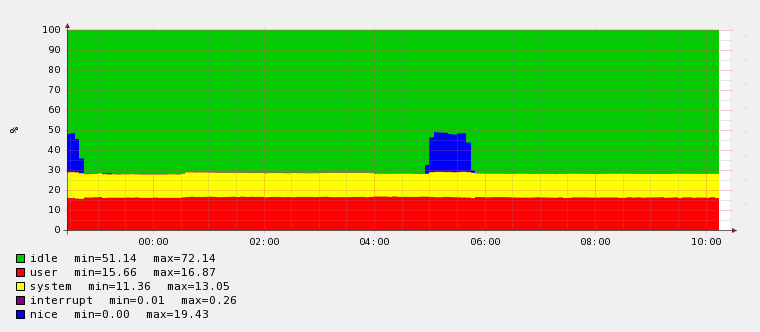
\includegraphics[scale=0.36]{pics/cpu-12h.eps}
	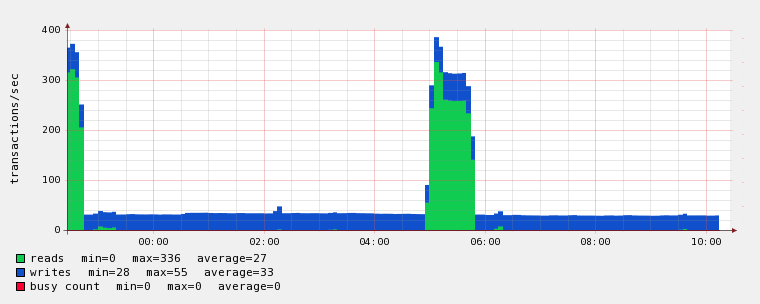
\includegraphics[scale=0.36]{pics/disk-io-12h.eps} \\
	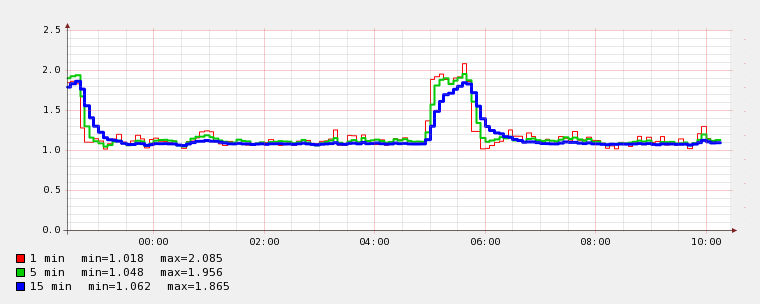
\includegraphics[scale=0.36]{pics/load-average-12h.eps}
	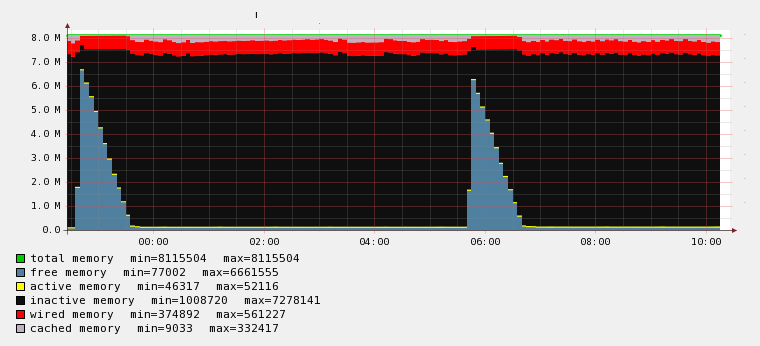
\includegraphics[scale=0.36]{pics/memory-12h.eps} \\
\end{center}

\subsection{Know your systems.}
CPU load - 12 hours
\begin{center}
	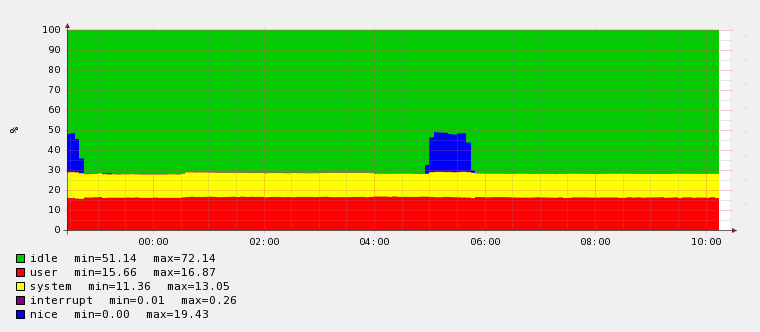
\includegraphics[scale=0.9]{pics/cpu-12h.eps}
\end{center}

\subsection{Know your systems.}
Disk I/O - 12 hours
\begin{center}
	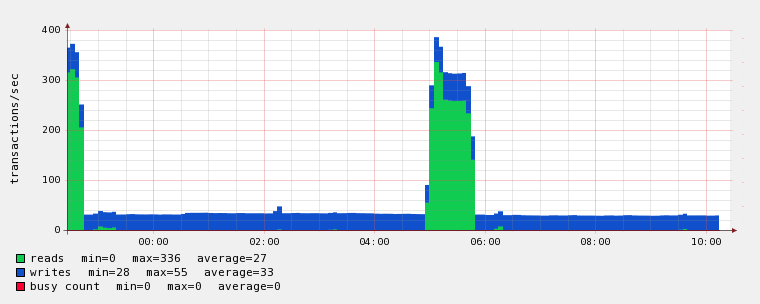
\includegraphics[scale=0.9]{pics/disk-io-12h.eps}
\end{center}

\subsection{Know your systems.}
Load Average - 12 hours
\begin{center}
	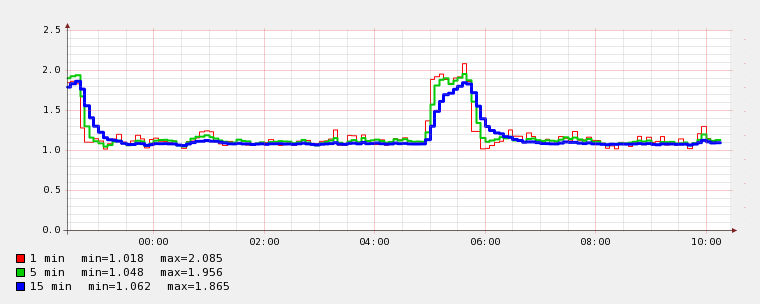
\includegraphics[scale=0.9]{pics/load-average-12h.eps}
\end{center}

\subsection{Know your systems.}
Memory - 12 hours
\begin{center}
	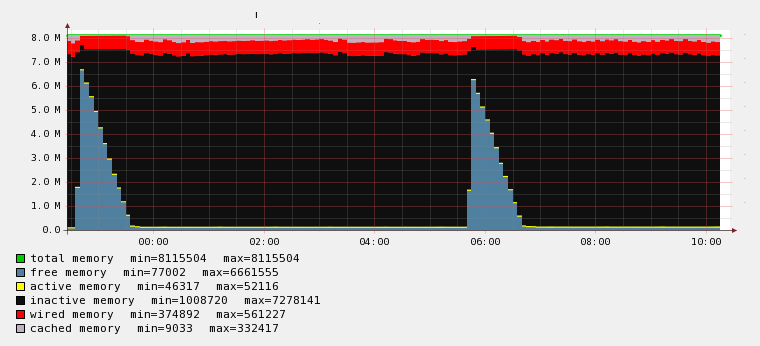
\includegraphics[scale=0.9]{pics/memory-12h.eps}
\end{center}

\subsection{Know your systems.}
12 hours
\begin{center}
	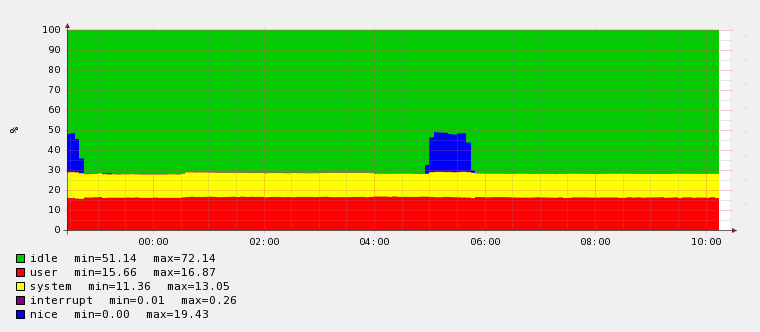
\includegraphics[scale=0.36]{pics/cpu-12h.eps}
	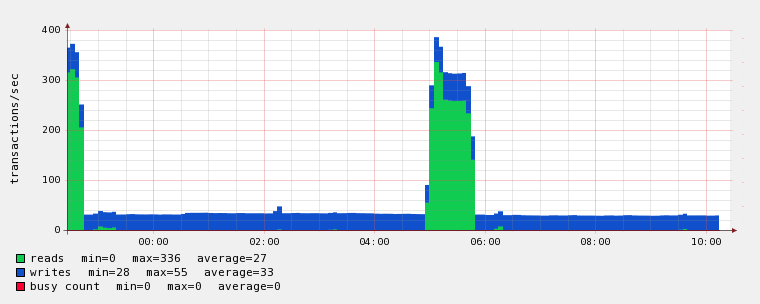
\includegraphics[scale=0.36]{pics/disk-io-12h.eps} \\
	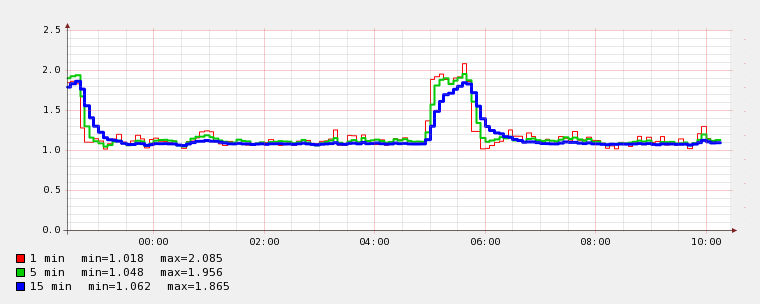
\includegraphics[scale=0.36]{pics/load-average-12h.eps}
	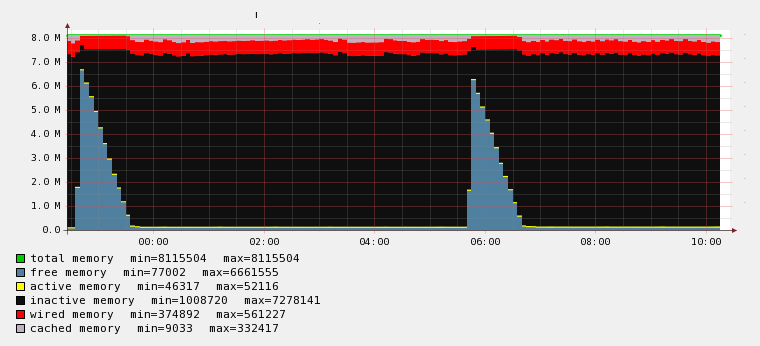
\includegraphics[scale=0.36]{pics/memory-12h.eps} \\
\end{center}

\subsection{Know your systems.}
7 days
\begin{center}
	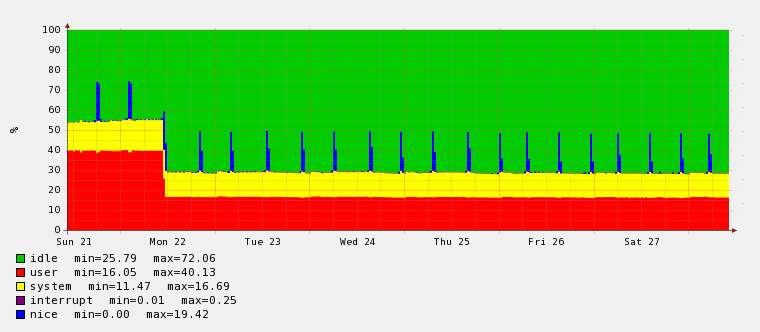
\includegraphics[scale=0.36]{pics/cpu-7day.eps}
	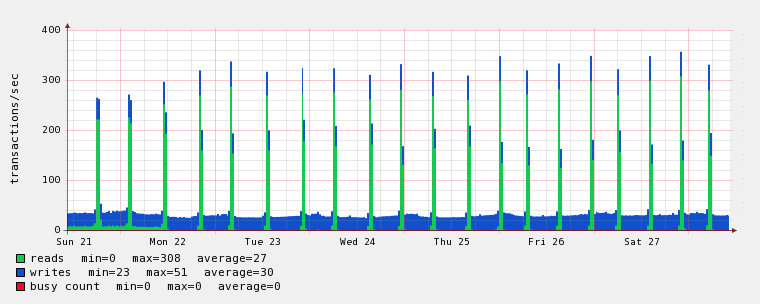
\includegraphics[scale=0.36]{pics/disk-io-7day.eps} \\
	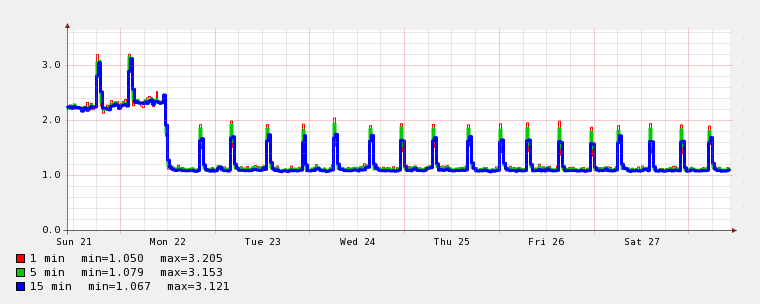
\includegraphics[scale=0.36]{pics/load-average-7day.eps}
	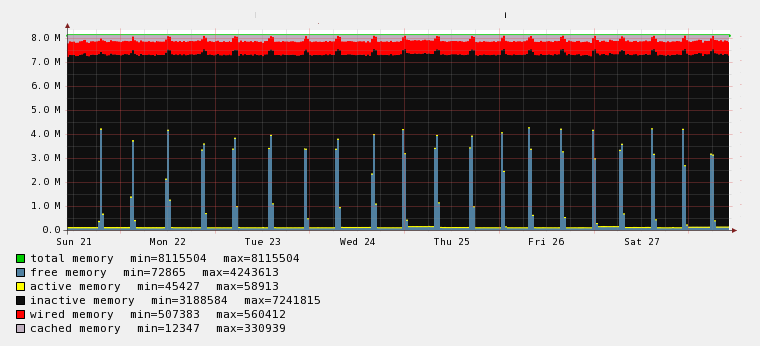
\includegraphics[scale=0.36]{pics/memory-7day.eps} \\
\end{center}



%\subsection{Know your systems.}
%CPU load - 7 days
%\begin{center}
%	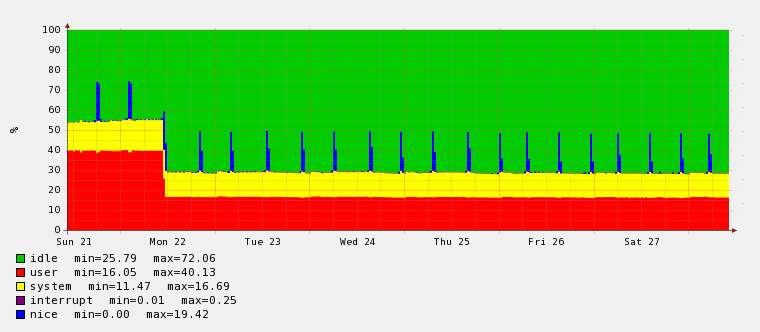
\includegraphics[scale=0.9]{pics/cpu-7day.eps}
%\end{center}
%
%\subsection{Know your systems.}
%Disk I/O - 7 days
%\begin{center}
%	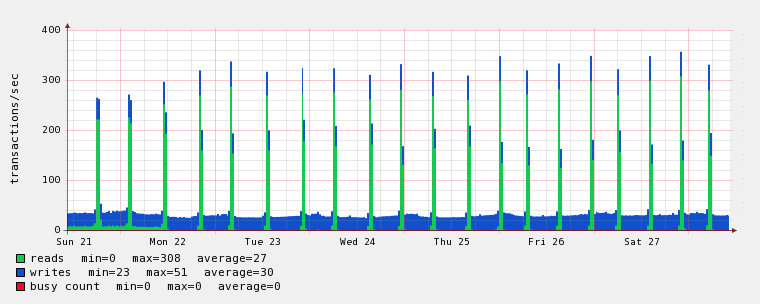
\includegraphics[scale=0.9]{pics/disk-io-7day.eps}
%\end{center}
%
%\subsection{Know your systems.}
%Load Average - 7 days
%\begin{center}
%	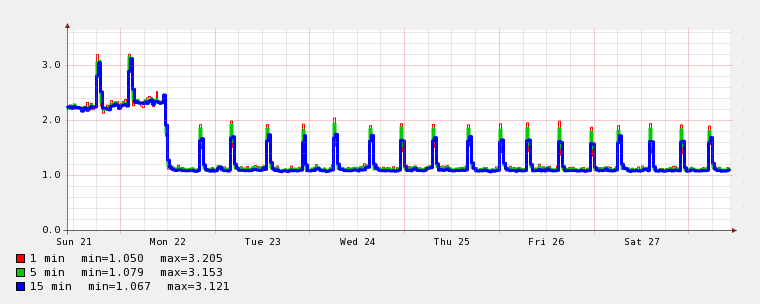
\includegraphics[scale=0.9]{pics/load-average-7day.eps}
%\end{center}
%
%\subsection{Know your systems.}
%Memory - 7 days
%\begin{center}
%	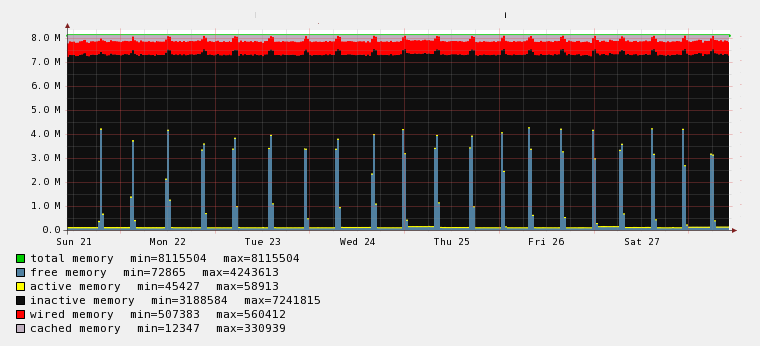
\includegraphics[scale=0.9]{pics/memory-7day.eps}
%\end{center}
%
%
\subsection{Know your systems.}
30 days
\begin{center}
	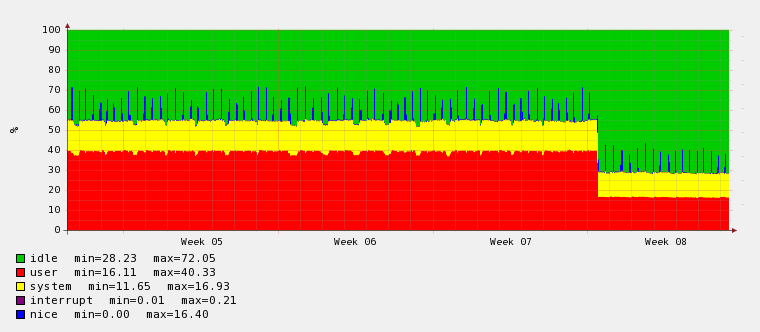
\includegraphics[scale=0.36]{pics/cpu-30day.eps}
	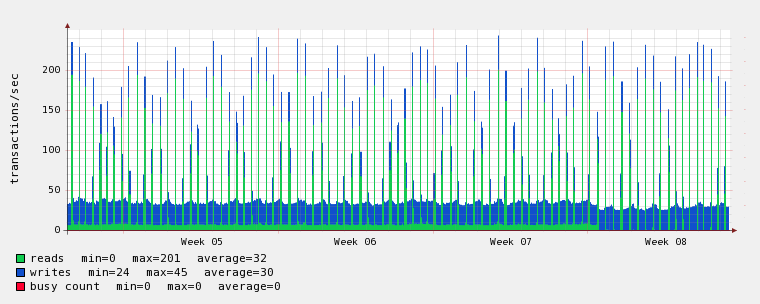
\includegraphics[scale=0.36]{pics/disk-io-30day.eps} \\
	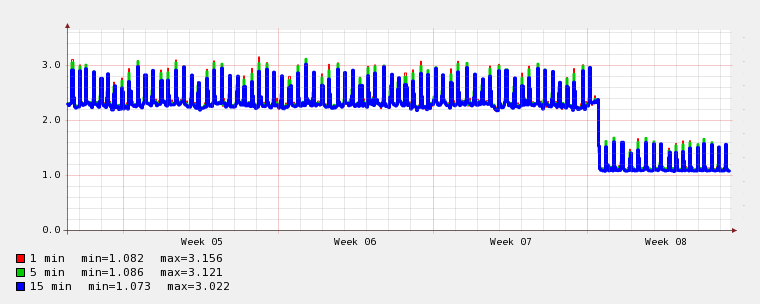
\includegraphics[scale=0.36]{pics/load-average-30day.eps}
	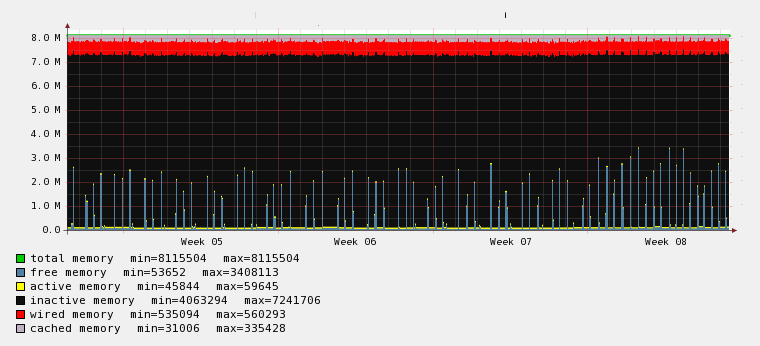
\includegraphics[scale=0.36]{pics/memory-30day.eps} \\
\end{center}


\subsection{Know your systems.}
CPU load - 30 days
\begin{center}
	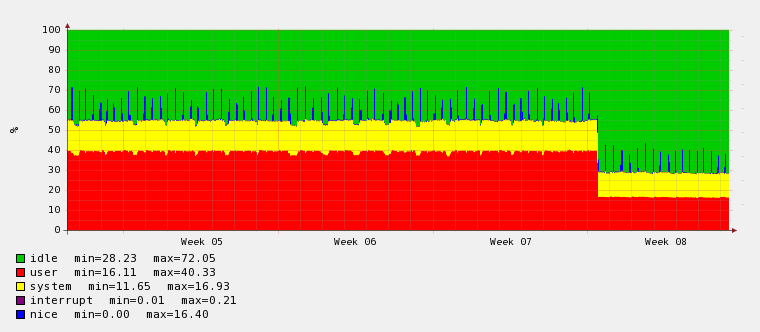
\includegraphics[scale=0.9]{pics/cpu-30day.eps}
\end{center}

%\subsection{Know your systems.}
%Disk I/O - 30 days
%\begin{center}
%	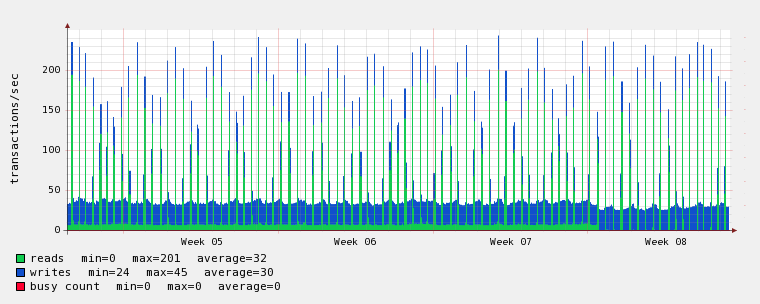
\includegraphics[scale=0.9]{pics/disk-io-30day.eps}
%\end{center}
%
\subsection{Know your systems.}
Load Average - 30 days
\begin{center}
	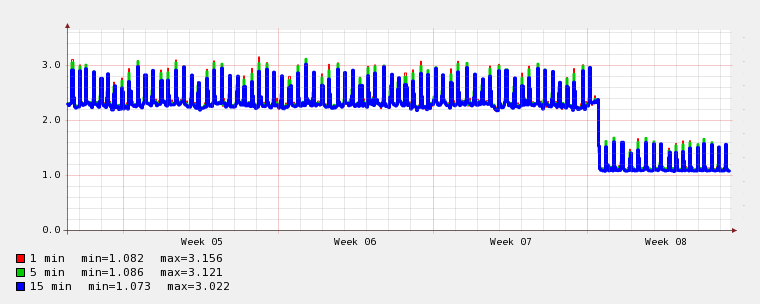
\includegraphics[scale=0.9]{pics/load-average-30day.eps}
\end{center}

%\subsection{Know your systems.}
%Memory - 30 days
%\begin{center}
%	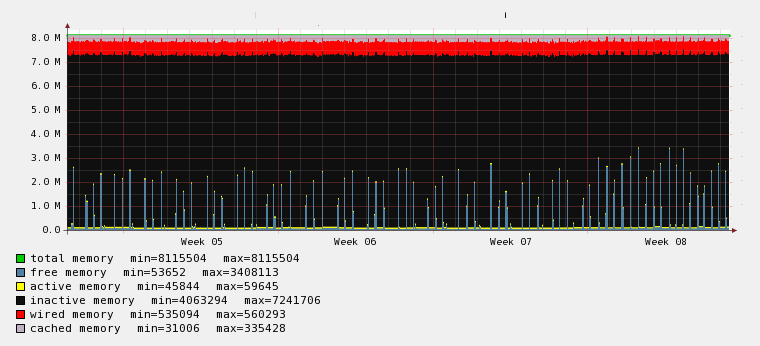
\includegraphics[scale=0.9]{pics/memory-30day.eps}
%\end{center}

%\subsection{Know your systems.}
%30 days
%\begin{center}
%	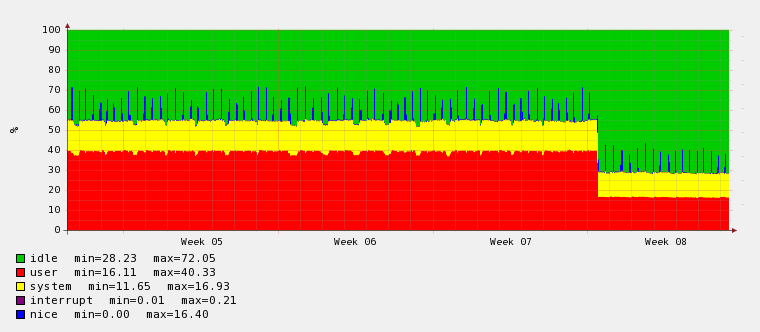
\includegraphics[scale=0.36]{pics/cpu-30day.eps}
%	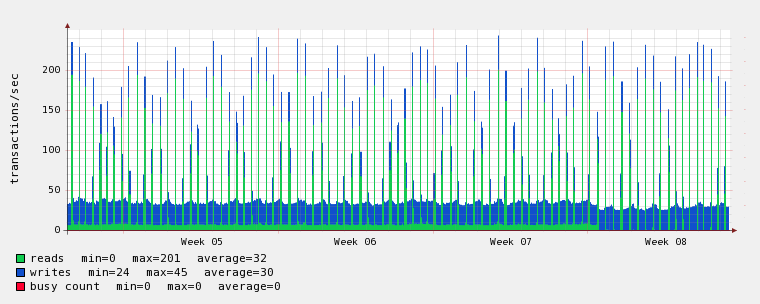
\includegraphics[scale=0.36]{pics/disk-io-30day.eps} \\
%	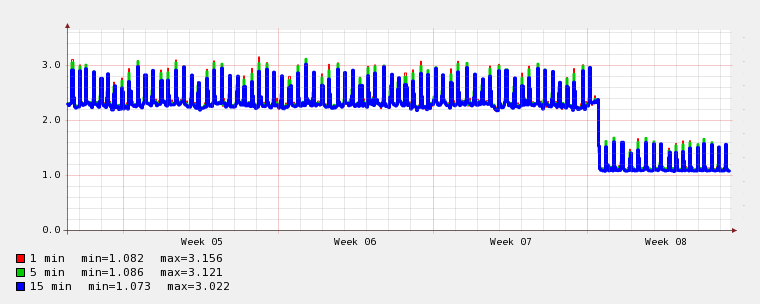
\includegraphics[scale=0.36]{pics/load-average-30day.eps}
%	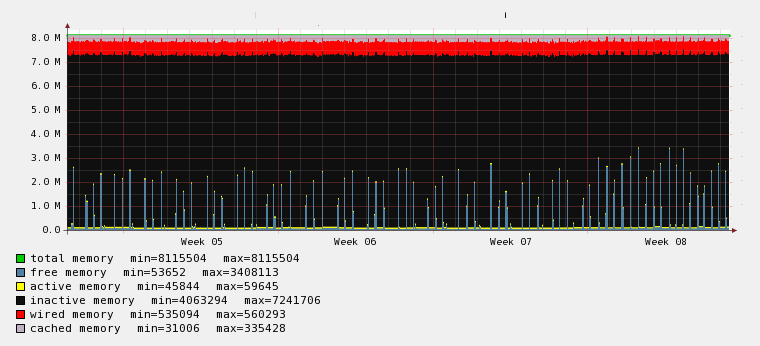
\includegraphics[scale=0.36]{pics/memory-30day.eps} \\
%\end{center}
%
%



\subsection{Remedy}
If you don't have enough of something, you have very few options:
\\

\begin{center}
	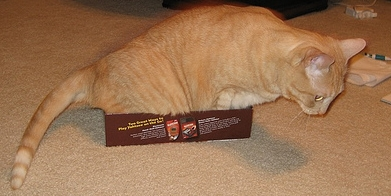
\includegraphics[scale=0.9]{pics/cat_in_box.eps}
\end{center}

\subsection{Remedy}
If you don't have enough of something, you have very few options:
\\

You can get more of it.

\begin{center}
	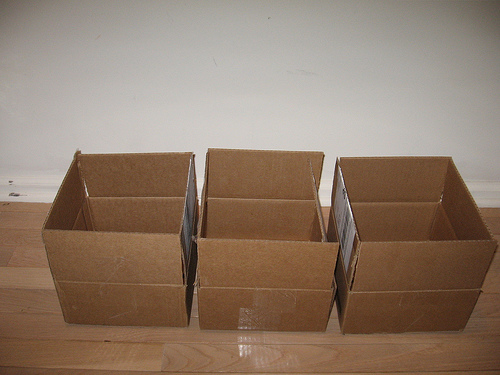
\includegraphics[scale=0.7]{pics/boxes2.eps}
\end{center}

\subsection{Remedy}
If you don't have enough of something, you have very few options:
\\

You can use less of it.

\begin{center}
	
\includegraphics[scale=0.7]{pics/small_cat.eps}
\end{center}

\subsection{Remedy}
If you don't have enough of something, you have very few options:
\\

You can ration / distribute the amount you do have.

\begin{center}
	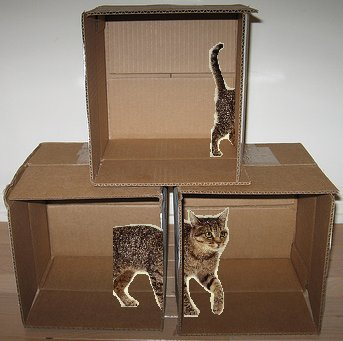
\includegraphics[scale=0.8]{pics/boxes.eps}
\end{center}

\subsection{Monitoring CPU Workload}
System Load Average: average number of processes in a kernel's run queue. \\

\vspace*{\fill}
\verb+up 1318 days, 13:46, 1 user, load averages: 993.81, 272.91, 1012.18+\\
\verb+up    4 days, 18:28, 0 users, load averages: 70.54, 51.09, 47.18+\\
\verb+up    8 days, 23:05, 0 users, load averages: 7.07, 16.89, 20.28+\\
\verb+up  314 days, 44 mins, 0 users, load averages: 2.78, 3.97, 3.88+ \\
\vspace*{\fill}

\subsection{Managing CPU Workload}
Things you can do to keep processes under control:
\begin{itemize}
	\item ``get more of it'':
		\begin{itemize}
			\item get faster CPUs
			\item get more CPUs (per host)
			\item get more hosts
		\end{itemize}
\end{itemize}

\subsection{Managing CPU Workload}
Things you can do to keep processes under control:
\begin{itemize}
	\item ``use less of it'':
		\begin{itemize}
			\item optimize programs
			\item restrict certain CPUs for specific usage (\verb+cpuset(1)+)
			\item change a process's priorities (\verb+nice(1)+ and
				\verb+renice(1)+)
			\item create system-wide CPU limits (\verb+ulimit+)
			\item suspend and/or kill processes
		\end{itemize}
\end{itemize}

\subsection{Managing CPU Workload}
Things you can do to keep processes under control:
\begin{itemize}
	\item ``ration / redistribute the amount you have'':
		\begin{itemize}
			\item schedule processes at off-hours
			\item rewrite program(s) to use multithreading
			\item parallelize program(s) across multiple hosts
		\end{itemize}
\end{itemize}


%\subsection{Memory Performance}
%Things to consider:
%\begin{itemize}
%	\item {\em paging} vs. {\em swapping}
%	\item monitoring memory usage with \verb+vmstat(1)+ and \verb+sar(1)+
%	\item use of \verb+ulimit+ (or \verb+limit+) to set the stacksize,
%		datasize, memorysize
%	\item adjust buffer cache
%	\item managing swap area
%\end{itemize}
%
%\subsection{Disk Performance}
%Mostly covered in previous lecture.  To summarize:
%\begin{itemize}
%	\item hardware limitations
%	\item filesystem usage
%	\item I/O subsystem configuration
%	\item filesystem housekeeping
%\end{itemize}
%

\subsection{Words of Wisdom}
\\

\newcommand{\gargantuan}{\fontsize{60}{65}\selectfont}
\gargantuan
\begin{center}
Don't try to fix \\
what isn't broken.
\end{center}
\Normalsize

%\subsection{So many knobs...}
%\begin{verbatim}
%$ sysctl -a
%kern.maxproc = 148
%kern.maxfiles = 548
%kern.ngroups = 16
%kern.iov_max = 1024
%kern.mbuf.msize = 256
%kern.mbuf.mclbytes = 2048
%kern.mbuf.nmbclusters = 1024
%kern.mbuf.mblowat = 16
%kern.mbuf.mcllowat = 8
%vm.nkmempages = 32768
%vm.bufcache = 15
%vm.bufmem = 11900928
%vm.bufmem_lowater = 9876480
%vm.bufmem_hiwater = 79011840
%net.inet.tcp.sendspace = 32768
%net.inet.tcp.recvspace = 32768
%\end{verbatim}
%
%\subsection{So many knobs...}
%\begin{verbatim}
%$ man 4 options
%options MAXUSERS=integer
%options MAXUPRC=integer
%options NOFILE=integer
%options MAXFILES=integer
%options TCP_SENDSPACE=value
%options TCP_RECVSPACE=value
%options TCP_INIT_WIN=value
%options SYSVSHM
%options SHMMAXPGS=value
%options NMBCLUSTERS=value
%options NKMEMPAGES=value
%options BUFPAGES=value
%options MAXTSIZ=bytes
%options DFLDSIZ=bytes
%options LIMITMEM=value
%options NVNODE=integer
%\end{verbatim}
%
\newpage
\vspace*{\fill}
\begin{center}
    \Hugesize
        Hooray! \\ [1em]
    \hspace*{5mm}
    \blueline\\
    \hspace*{5mm}\\
        5 Minute Break
\end{center}
\vspace*{\fill}

\newpage
\vspace*{\fill}
\begin{center}
	\Hugesize
		Popular Services \\ [1em]
	\hspace*{5mm}
	\blueline\\
	\hspace*{5mm}\\
		Simple Mail Transfer Protocol
\end{center}
\vspace*{\fill}

\subsection{Email... still popular}
\begin{itemize}
	\item {\bf 90 trillion} – The number of emails sent on the Internet in 2009.
	\item {\bf 247 billion} – Average number of email messages per day.
	\item {\bf 1.4 billion} – The number of email users worldwide.
	\item {\bf 100 million} – New email users since the year before.
	\item {\bf 81\%} – The percentage of emails that were spam.
	\item {\bf 92\%} – Peak spam levels late in the year.
	\item {\bf 24\%} – Increase in spam since last year.
	\item {\bf 200 billion} – The number of spam emails per day (assuming 81\% are spam).
\end{itemize}

\subsection{The Mail System}
Divided into
\begin{itemize}
	\item {\em Mail User Agent} or MUA, such as {\em mutt}
	\item {\em Mail Transfer Agent} or MTA, such as {\em postfix}
	\item {\em Mail Delivery Agent} or MDA, such as {\em procmail}
	\item {\em Access Agent} providing access via {\em POP}, {\em IMAP} etc.
\end{itemize}


\subsection{Sending email}
\begin{verbatim}
$ mail -s "Act I, Scene I" jschauma@cs.stevens.edu
When shall we three meet again?
In thunder, lightning, or in rain?
.
EOT
$
\end{verbatim}

\subsection{Anatomy of an email message}
An email consists of:
\begin{itemize}
	\item mandatory headers (such as "From ", "Delivered-To: ", ...)
	\item optional headers (such as "From: ", "To: ", "Subject: ", ...)
	\item the (optional) body of the message
\end{itemize}

\subsection{Anatomy of an email message}
\begin{verbatim}
Date: Sun, 27 Mar 2011 18:54:04 -0400 (EDT)
From: Jan Schaumann <jschauma@netmeister.org>
To: jschauma@cs.stevens.edu
Subject: Act I, Scene I

When shall we three meet again?
In thunder, lightning, or in rain?

\end{verbatim}

\subsection{Anatomy of an email message}
\small
\begin{verbatim}
From jschauma@cs.stevens.edu  Sun Mar 18 22:48:09 2012
Return-Path: jschauma@cs.stevens.edu
X-Original-To: jschauma@netmeister.org
Delivered-To: jschauma@netmeister.org
Received: by panix.netmeister.org (Postfix, from userid 1004)
        id 93A29356BC1; Sun, 18 Mar 2012 22:48:09 -0400 (EDT)
Received: from na3sys009aog108.obsmtp.com (na3sys009aog108.obsmtp.com [74.125.149.199])
        by panix.netmeister.org (Postfix) with SMTP id 69B91356BBB
        for <jschauma@netmeister.org>; Sun, 18 Mar 2012 22:47:49 -0400 (EDT)
Received: from warp.stevens.edu ([155.246.14.14]) by na3sys009aob108.postini.com ([74.125.148.12])
        with SMTP ID DSNKT2aeVJEJy0AYQcjXfWII8P62lyoYXAFm@postini.com; Sun, 18 Mar 2012 19:48:08 PDT
Received: from psmtp.com (na3sys009amx209.postini.com [74.125.149.49])
        by warp.stevens.edu (Postfix) with SMTP id 168646041A
        for <jschauma@cs.stevens.edu>; Sun, 18 Mar 2012 22:47:36 -0400 (EDT)
Received: from eva.srcit.stevens-tech.edu ([155.246.89.108]) by na3sys009amx209.postini.com
        ([74.125.148.10]) with SMTP; Sun, 18 Mar 2012 21:47:39 CDT
Subject: Act I, Scene I
X-pstn-neptune: 0/0/0.00/0
X-pstn-levels:     (S:30.88262/99.90000 CV:99.9000 FC:95.5390 LC:95.5390
R:95.9108 P:95.9108
        M:97.0282 C:98.6951 )
X-pstn-dkim: 0 skipped:no-from
Message-ID: <2615178024788798087302160308530@psmtp.com>
X-pstn-settings: 3 (1.0000:1.0000) s cv gt3 gt2 gt1
X-pstn-addresses: from <jschauma@cs.stevens.edu> [db-null]
Date: Sun, 18 Mar 2012 22:47:36 -0400 (EDT)
From: jschauma@cs.stevens.edu
To: undisclosed-recipients: ;

When shall we three meet again?
In thunder, lightning, or in rain?
\end{verbatim}
\Normalsize

\subsection{Sending email}
\begin{verbatim}
$ mail -s "Act I, Scene I" jschauma@cs.stevens.edu
When shall we three meet again?
In thunder, lightning, or in rain?
.
EOT
$
\end{verbatim}

\subsection{Who to hand the mail to?}
\newcommand{\smallish}{\fontsize{16}{16}\selectfont}
\begin{verbatim}
$ host -t mx cs.stevens.edu
cs.stevens.edu mail is handled by 20 stevens.edu.s9a2.psmtp.com.
cs.stevens.edu mail is handled by 30 stevens.edu.s9b1.psmtp.com.
cs.stevens.edu mail is handled by 10 stevens.edu.s9a1.psmtp.com.
cs.stevens.edu mail is handled by 40 stevens.edu.s9b2.psmtp.com.
$
\end{verbatim}
\Normalsize

\subsection{In more detail...}
Finding the right mail server to talk to:
\begin{verbatim}
IP 166.84.7.99.52299 > 166.84.67.2.53: 53739+ MX? cs.stevens.edu. (32)
IP 166.84.67.2.53 > 166.84.7.99.52299: 53739 4/2/6 MX[|domain]
IP 166.84.7.99.52298 > 166.84.67.2.53: 53740+ A? stevens.edu.s9a1.psmtp.com. (44)
IP 166.84.67.2.53 > 166.84.7.99.52298: 53740 1/4/4 (203)
IP 166.84.7.99.52297 > 166.84.67.2.53: 53741+ AAAA? stevens.edu.s9a1.psmtp.com. (44)
IP 166.84.67.2.53 > 166.84.7.99.52297: 53741 0/1/0 (110)
\end{verbatim}
\Normalsize

\subsection{By the way...}
\begin{verbatim}
$ dig stevens.edu.s9a1.psmtp.com.
;; ANSWER SECTION:
stevens.edu.s9a1.psmtp.com. 12564 IN    A       74.125.148.10

;; AUTHORITY SECTION:
psmtp.com.              31973   IN      NS      ns3.google.com.
psmtp.com.              31973   IN      NS      ns4.google.com.
psmtp.com.              31973   IN      NS      ns2.google.com.
psmtp.com.              31973   IN      NS      ns1.google.com.

;; ADDITIONAL SECTION:
ns1.google.com.         296322  IN      A       216.239.32.10
ns2.google.com.         321381  IN      A       216.239.34.10
ns3.google.com.         329449  IN      A       216.239.36.10
ns4.google.com.         321381  IN      A       216.239.38.10
[...]
\end{verbatim}

\subsection{Sending mail...}
\smallish
\begin{verbatim}
$ telnet stevens.edu.s9a1.psmtp.com 25
Trying 74.125.148.10...
Connected to stevens.edu.s9a1.psmtp.com.
Escape character is '^]'.
220 Postini ESMTP 202 y6_37_0c5 ready.  CA Business and Professions Code
Section 17538.45 forbids use of this system for unsolicited electronic
mail advertisements.
helo panix.netmeister.org
250 Postini says hello back
mail from: <jschauma@netmeister.org>
250 Ok
rcpt to: <jschauma@cs.stevens.edu>
250 Ok
data
354 Feed me
Subject: Act I, Scene I

When shall we three meet again?
In thunder, lightning, or in rain?
.
250 Thanks
quit
221 Catch you later
Connection closed by foreign host.
\end{verbatim}
\Normalsize

\subsection{Sending the mail}
\begin{verbatim}
IP 166.84.7.99.51845 > 74.125.148.10.25: S 404385236:404385236(0)
IP 74.125.148.10.25 > 166.84.7.99.51845: S 1228051958:1228051958(0) ack 404385237
IP 166.84.7.99.51845 > 74.125.148.10.25: . ack 1
IP 74.125.148.10.25 > 166.84.7.99.51845: P 1:170(169) ack 1
IP 166.84.7.99.51845 > 74.125.148.10.25: P 1:28(27) ack 170
IP 74.125.148.10.25 > 166.84.7.99.51845: . ack 28
[...]
IP 74.125.148.10.25 > 166.84.7.99.51845: . ack 508
IP 74.125.148.10.25 > 166.84.7.99.51845: P 266:278(12) ack 508
IP 166.84.7.99.51845 > 74.125.148.10.25: P 508:514(6) ack 278
IP 166.84.7.99.51845 > 74.125.148.10.25: F 514:514(0) ack 278
IP 74.125.148.10.25 > 166.84.7.99.51845: . ack 514
IP 74.125.148.10.25 > 166.84.7.99.51845: P 278:299(21) ack 514
IP 74.125.148.10.25 > 166.84.7.99.51845: F 299:299(0) ack 514
IP 74.125.148.10.25 > 166.84.7.99.51845: . ack 515
\end{verbatim}
\Normalsize

\subsection{SMTP Codes}
SMTP codes consist of three digits in five classes:
\begin{itemize}
	\item {\bf 1xx} --  Mail server has accepted the command, but does not yet
		take any action. A confirmation message is required.
	\item {\bf 2xx} --  Mail server has completed the task successfully
		without errors.
	\item {\bf 3xx} --  Mail server has understood the request, but requires
		further information to complete it.
	\item {\bf 4xx} --  Mail server has encountered a temporary failure. If
		the command is repeated without any change, it might be
		completed. Try again, it may help!
	\item {\bf 5xx} --  Mail server has encountered a fatal error. Your
		request can't be processed.
\end{itemize}

\subsection{Receiving the mail}
\begin{verbatim}

IP 74.125.149.69.59141 > 166.84.7.99.25: S 1919605344:1919605344(0)
IP 166.84.7.99.25 > 74.125.149.69.59141: S 472727490:472727490(0) ack 1919605345
IP 74.125.149.69.59141 > 166.84.7.99.25: . ack 1
IP 166.84.7.99.52290 > 166.84.67.2.53: 10348+ PTR? 69.149.125.74.in-addr.arpa. (44)
IP 166.84.67.2.53 > 166.84.7.99.52290: 10348 1/4/4 (227)
IP 166.84.7.99.52289 > 166.84.67.2.53: 10349+ AAAA? na3sys009aog102.obsmtp.com. (44)
IP 166.84.67.2.53 > 166.84.7.99.52289: 10349 0/1/0 (110)
IP 166.84.7.99.52288 > 166.84.67.2.53: 10350+ A? na3sys009aog102.obsmtp.com. (44)
IP 166.84.67.2.53 > 166.84.7.99.52288: 10350 1/4/4 (203)
IP 166.84.7.99.25 > 74.125.149.69.59141: P 1:41(40) ack 1
IP 74.125.149.69.59141 > 166.84.7.99.25: . ack 41
[...]
IP 74.125.149.69.59141 > 166.84.7.99.25: P 71:106(35) ack 81
IP 166.84.7.99.52287 > 166.84.67.2.53: 10351+ A? na3sys009aog102.obsmtp.com. (44)
IP 166.84.67.2.53 > 166.84.7.99.52287: 10351 1/4/4 (203)
IP 166.84.7.99.52286 > 166.84.67.2.53: 10352+ A? 69.149.125.74.sbl.spamhaus.org. (48)
IP 166.84.67.2.53 > 166.84.7.99.52286: 10352 NXDomain 0/1/0 (104)
IP 166.84.7.99.52285 > 166.84.67.2.53: 10353+ A? 69.149.125.74.bl.spamcop.net. (46)
IP 166.84.67.2.53 > 166.84.7.99.52285: 10353 NXDomain 0/1/0 (99)
IP 166.84.7.99.25 > 74.125.149.69.59141: P 81:95(14) ack 106
IP 74.125.149.69.59141 > 166.84.7.99.25: . ack 95
IP 74.125.149.69.59141 > 166.84.7.99.25: P 106:112(6) ack 95
IP 166.84.7.99.25 > 74.125.149.69.59141: P 95:132(37) ack 112
IP 74.125.149.69.59141 > 166.84.7.99.25: . ack 132
IP 74.125.149.69.59141 > 166.84.7.99.25: P 112:1276(1164) ack 132
IP 166.84.7.99.25 > 74.125.149.69.59141: . ack 1276
IP 74.125.149.69.59141 > 166.84.7.99.25: P 1276:1348(72) ack 132
IP 166.84.7.99.25 > 74.125.149.69.59141: P 132:169(37) ack 1348
IP 166.84.7.99.25 > 74.125.149.69.59141: P 169:184(15) ack 1354
IP 166.84.7.99.25 > 74.125.149.69.59141: F 184:184(0) ack 1354
IP 74.125.149.69.59141 > 166.84.7.99.25: F 1354:1354(0) ack 184
IP 166.84.7.99.25 > 74.125.149.69.59141: . ack 1355
IP 74.125.149.69.59141 > 166.84.7.99.25: . ack 185
\end{verbatim}
\Normalsize

\subsection{Temporary Failures}
\begin{verbatim}
Mar  4 18:20:29 <mail.info>panix postfix/smtpd[22818]: NOQUEUE: reject:
RCPT from na3sys009aog115.obsmtp.com[74.125.149.238]: 450 4.1.8
<apache@underdog.stevens.edu>: Sender address rejected: Domain not found;
from=<apache@underdog.stevens.edu> to=<jschauma@netmeister.org> proto=SMTP
helo=<na3sys009aog115.obsmtp.com>
Mar  4 18:20:29 <mail.info>panix postfix/smtpd[26666]: NOQUEUE: reject:
RCPT from na3sys009aog130.obsmtp.com[74.125.149.143]: 450 4.1.8
<apache@underdog.stevens.edu>: Sender address rejected: Domain not found;
from=<apache@underdog.stevens.edu> to=<jschauma@netmeister.org> proto=SMTP
helo=<na3sys009aog130.obsmtp.com>
Mar  4 18:23:23 <mail.info>panix postfix/smtpd[22818]: NOQUEUE: reject:
RCPT from na3sys009aog136.obsmtp.com[74.125.149.85]: 450 4.1.8
<apache@underdog.stevens.edu>: Sender address rejected: Domain not found;
from=<apache@underdog.stevens.edu> to=<jschauma@netmeister.org> proto=SMTP
helo=<na3sys009aog136.obsmtp.com>
\end{verbatim}

\subsection{Service Considerations}

\begin{itemize}
	\item outsourcing versus in-house
	\item mail delivery cannons for notifications vs. spam lists
	\item high volume traffic demands fine-tuned systems
	\item high volume traffic implications on logging
	\item privacy considerations
\end{itemize}

\subsection{HW5}

Have a presentation topic discussed and agreed upon with me by next
week.
\\

\verb+http://www.cs.stevens.edu/~jschauma/615/s13-hw5.html+


\subsection{Reading}
Processes:
\begin{itemize}
	\item \verb+fork(2)+ and \verb+exec(2)+
	\item \verb+http://www.cse.fau.edu/~roy/cop4604.02s/notes/process.html+
\end{itemize}
System Activity Monitoring:
\begin{itemize}
	\item \verb+systat(1)+, \verb+ps(1)+, \verb+vmstat(1)+ et al
\end{itemize}
Managing/Monitoring CPU Workload:
\begin{itemize}
	\item \verb+at(1)+ and \verb+batch(1)+
	\item \verb+cpuset(1)+
	\item \verb+nice(1)+
\end{itemize}
Various kernel tuning:
\begin{itemize}
	\item \verb+options(4)+
	\item \verb+http://www.netbsd.org/guide/en/chap-tuning.html+
\end{itemize}

\subsection{Reading}
SMTP:
\begin{itemize}
	\item \verb+http://bit.ly/5zIadJ+
	\item RFC 821, 2821
	\item \verb+aliases(5)+, \verb+mail(1)+
	\item \verb+sendmail(8)+, \verb+postfix(8)+
\end{itemize}

\end{document}
